% Options for packages loaded elsewhere
\PassOptionsToPackage{unicode}{hyperref}
\PassOptionsToPackage{hyphens}{url}
%
\documentclass[
  9pt,
  ignorenonframetext,
]{beamer}
\usepackage{pgfpages}
% set the section number 
\setbeamertemplate{section in toc}[sections numbered]
\setbeamertemplate{subsection in toc}[subsections numbered]
\setbeamertemplate{navigation symbols}{}
% set the page
\setbeamertemplate{footline}[page number]
\setbeamertemplate{caption}[numbered]
\setbeamertemplate{caption label separator}{: }
\setbeamercolor{caption name}{fg=normal text.fg}
\beamertemplatenavigationsymbolsempty

%%
%%% Definition of colors
%%% Source: https://latexcolor.com/
\definecolor{blanchedalmond}{rgb}{1.0, 0.92, 0.8}
\definecolor{blond}{rgb}{0.98, 0.94, 0.75}
%%% End of definition of colors
%%

% Prevent slide breaks in the middle of a paragraph
\widowpenalties 1 10000
\raggedbottom
\setbeamertemplate{part page}{
  \centering
  \begin{beamercolorbox}[sep=16pt,center]{part title}
    \usebeamerfont{part title}\insertpart\par
  \end{beamercolorbox}
}
\setbeamertemplate{section page}{
  \centering
  \begin{beamercolorbox}[sep=12pt,center]{part title}
    \usebeamerfont{section title}\insertsection\par
  \end{beamercolorbox}
}
\setbeamertemplate{subsection page}{
  \centering
  \begin{beamercolorbox}[sep=8pt,center]{part title}
    \usebeamerfont{subsection title}\insertsubsection\par
  \end{beamercolorbox}
}
\AtBeginPart{
  \frame{\partpage}
}
\AtBeginSection{
  \ifbibliography
  \else
    \frame{\sectionpage}
  \fi
}
\AtBeginSubsection{
  \frame{\subsectionpage}
}
\usepackage{lmodern}
\usepackage{amssymb,amsmath}
\usepackage{ifxetex,ifluatex}
\ifnum 0\ifxetex 1\fi\ifluatex 1\fi=0 % if pdftex
  \usepackage[T1]{fontenc}
  \usepackage[utf8]{inputenc}
  \usepackage{textcomp} % provide euro and other symbols
\else % if luatex or xetex
  \usepackage{unicode-math}
  \defaultfontfeatures{Scale=MatchLowercase}
  \defaultfontfeatures[\rmfamily]{Ligatures=TeX,Scale=1}
\fi
\usetheme[]{Goettingen}
\usecolortheme{rose}
% Use upquote if available, for straight quotes in verbatim environments
\IfFileExists{upquote.sty}{\usepackage{upquote}}{}
\IfFileExists{microtype.sty}{% use microtype if available
  \usepackage[]{microtype}
  \UseMicrotypeSet[protrusion]{basicmath} % disable protrusion for tt fonts
}{}
\makeatletter
\@ifundefined{KOMAClassName}{% if non-KOMA class
  \IfFileExists{parskip.sty}{%
    \usepackage{parskip}
  }{% else
    \setlength{\parindent}{0pt}
    \setlength{\parskip}{6pt plus 2pt minus 1pt}}
}{% if KOMA class
  \KOMAoptions{parskip=half}}
  
% adjust for sidebar
  \setbeamertemplate{sidebar \beamer@sidebarside}
  {
    \beamer@tempdim=\beamer@sidebarwidth%
    \advance\beamer@tempdim by -6pt%
    \vskip4em%
    \insertverticalnavigation{\beamer@sidebarwidth}%
    \vfill
    \ifx\beamer@sidebarside\beamer@lefttext%
    \else%
      \usebeamercolor{normal text}%
      \llap{\usebeamertemplate***{navigation symbols}\hskip0.1cm}%
      \vskip2pt%
    \fi%
  }%

  \ifx\beamer@sidebarside\beamer@lefttext%
    \defbeamertemplate*{sidebar right}{sidebar theme}
    {%
      \vfill%
      \llap{\usebeamertemplate***{navigation symbols}\hskip0.1cm}%
      \vskip2pt}
  \fi

\setbeamertemplate{section in sidebar}%{sidebar theme}
{%
  \vbox{%
    \vskip1ex%
    \beamer@sidebarformat{3pt}{section in sidebar}{\insertsectionheadnumber
~\insertsectionhead}%
  }%
}
\setbeamertemplate{section in sidebar shaded}%{sidebar theme}
{%
  \vbox{%
    \vskip1ex%
    \beamer@sidebarformat{3pt}{section in sidebar shaded}{\insertsectionheadnumber
~\insertsectionhead}%
  }%
}  

\makeatother
\usepackage{xcolor}
\IfFileExists{xurl.sty}{\usepackage{xurl}}{} % add URL line breaks if available
\IfFileExists{bookmark.sty}{\usepackage{bookmark}}{\usepackage{hyperref}}
\hypersetup{
  pdftitle={L2: Graphs and Principal Component Analysis},
  pdfauthor={EJC},
  hidelinks,
  pdfcreator={LaTeX via pandoc}}
\urlstyle{same} % disable monospaced font for URLs
\newif\ifbibliography
\usepackage{color}
\usepackage{fancyvrb}
\newcommand{\VerbBar}{|}
\newcommand{\VERB}{\Verb[commandchars=\\\{\}]}
\DefineVerbatimEnvironment{Highlighting}{Verbatim}{commandchars=\\\{\}}
% Add ',fontsize=\small' for more characters per line
\usepackage{framed}
\definecolor{shadecolor}{RGB}{248,248,248}
\newenvironment{Shaded}{\begin{snugshade}}{\end{snugshade}}
\newcommand{\AlertTok}[1]{\textcolor[rgb]{0.94,0.16,0.16}{#1}}
\newcommand{\AnnotationTok}[1]{\textcolor[rgb]{0.56,0.35,0.01}{\textbf{\textit{#1}}}}
\newcommand{\AttributeTok}[1]{\textcolor[rgb]{0.77,0.63,0.00}{#1}}
\newcommand{\BaseNTok}[1]{\textcolor[rgb]{0.00,0.00,0.81}{#1}}
\newcommand{\BuiltInTok}[1]{#1}
\newcommand{\CharTok}[1]{\textcolor[rgb]{0.31,0.60,0.02}{#1}}
\newcommand{\CommentTok}[1]{\textcolor[rgb]{0.56,0.35,0.01}{\textit{#1}}}
\newcommand{\CommentVarTok}[1]{\textcolor[rgb]{0.56,0.35,0.01}{\textbf{\textit{#1}}}}
\newcommand{\ConstantTok}[1]{\textcolor[rgb]{0.00,0.00,0.00}{#1}}
\newcommand{\ControlFlowTok}[1]{\textcolor[rgb]{0.13,0.29,0.53}{\textbf{#1}}}
\newcommand{\DataTypeTok}[1]{\textcolor[rgb]{0.13,0.29,0.53}{#1}}
\newcommand{\DecValTok}[1]{\textcolor[rgb]{0.00,0.00,0.81}{#1}}
\newcommand{\DocumentationTok}[1]{\textcolor[rgb]{0.56,0.35,0.01}{\textbf{\textit{#1}}}}
\newcommand{\ErrorTok}[1]{\textcolor[rgb]{0.64,0.00,0.00}{\textbf{#1}}}
\newcommand{\ExtensionTok}[1]{#1}
\newcommand{\FloatTok}[1]{\textcolor[rgb]{0.00,0.00,0.81}{#1}}
\newcommand{\FunctionTok}[1]{\textcolor[rgb]{0.00,0.00,0.00}{#1}}
\newcommand{\ImportTok}[1]{#1}
\newcommand{\InformationTok}[1]{\textcolor[rgb]{0.56,0.35,0.01}{\textbf{\textit{#1}}}}
\newcommand{\KeywordTok}[1]{\textcolor[rgb]{0.13,0.29,0.53}{\textbf{#1}}}
\newcommand{\NormalTok}[1]{#1}
\newcommand{\OperatorTok}[1]{\textcolor[rgb]{0.81,0.36,0.00}{\textbf{#1}}}
\newcommand{\OtherTok}[1]{\textcolor[rgb]{0.56,0.35,0.01}{#1}}
\newcommand{\PreprocessorTok}[1]{\textcolor[rgb]{0.56,0.35,0.01}{\textit{#1}}}
\newcommand{\RegionMarkerTok}[1]{#1}
\newcommand{\SpecialCharTok}[1]{\textcolor[rgb]{0.00,0.00,0.00}{#1}}
\newcommand{\SpecialStringTok}[1]{\textcolor[rgb]{0.31,0.60,0.02}{#1}}
\newcommand{\StringTok}[1]{\textcolor[rgb]{0.31,0.60,0.02}{#1}}
\newcommand{\VariableTok}[1]{\textcolor[rgb]{0.00,0.00,0.00}{#1}}
\newcommand{\VerbatimStringTok}[1]{\textcolor[rgb]{0.31,0.60,0.02}{#1}}
\newcommand{\WarningTok}[1]{\textcolor[rgb]{0.56,0.35,0.01}{\textbf{\textit{#1}}}}
\usepackage{longtable,booktabs}
\usepackage{caption}
% Make caption package work with longtable
\makeatletter
\def\fnum@table{\tablename~\thetable}
\makeatother
\setlength{\emergencystretch}{3em} % prevent overfull lines
\providecommand{\tightlist}{%
  \setlength{\itemsep}{0pt}\setlength{\parskip}{0pt}}
\setcounter{secnumdepth}{-\maxdimen} % remove section numbering

%
% When using babel or polyglossia with biblatex, loading csquotes is recommended 
% to ensure that quoted texts are typeset according to the rules of your main language.
%
\usepackage{csquotes}

%
% blockquote
%
\definecolor{blockquote-border}{RGB}{221,221,221}
\definecolor{blockquote-text}{RGB}{89,89,89}
\usepackage{mdframed}
\newmdenv[rightline=false,bottomline=false,topline=false,linewidth=3pt,linecolor=blockquote-border,skipabove=\parskip]{customblockquote}
\renewenvironment{quote}{\begin{customblockquote}\list{}{\rightmargin=0em\leftmargin=0em}%
\item\relax\color{blockquote-text}\ignorespaces}{\unskip\unskip\endlist\end{customblockquote}}

%
% Source Sans Pro as the de­fault font fam­ily
% Source Code Pro for monospace text
%
% 'default' option sets the default 
% font family to Source Sans Pro, not \sfdefault.
%
\usepackage[default]{sourcesanspro}
\usepackage{sourcecodepro}

% XeLaTeX specific adjustments for straight quotes: https://tex.stackexchange.com/a/354887
% This issue is already fixed (see https://github.com/silkeh/latex-sourcecodepro/pull/5) but the 
% fix is still unreleased.
% TODO: Remove this workaround when the new version of sourcecodepro is reelased on CTAN.
\ifxetex
\makeatletter
\defaultfontfeatures[\ttfamily]
  { Numbers   = \sourcecodepro@figurestyle,
    Scale     = \SourceCodePro@scale,
    Extension = .otf }
\setmonofont
  [ UprightFont    = *-\sourcecodepro@regstyle,
    ItalicFont     = *-\sourcecodepro@regstyle It,
    BoldFont       = *-\sourcecodepro@boldstyle,
    BoldItalicFont = *-\sourcecodepro@boldstyle It ]
  {SourceCodePro}
\makeatother
\fi

\AtBeginSubsection{}
\AtBeginSection{}

\title{L2: Graphs and Principal Component Analysis}
\subtitle{BIOS6643}
\author{EJC}
\date{}
\institute{Department of Biostatistics \& Informatics, UCD Anschutz}

\begin{document}
\frame{\titlepage}

\begin{frame}
  \begin{columns}
  \column{10cm}
  \tableofcontents
  \end{columns}
\end{frame}
\begin{frame}{Learning objectives:}
\protect\hypertarget{learning-objectives}{}
\begin{enumerate}
\item
  Become familiar with multiple ways of representing longitudinal and
  cluster data.
\item
  Understand the basic ideas of principal component analysis
\end{enumerate}
\end{frame}

\hypertarget{introduction}{%
\section{Introduction}\label{introduction}}

\begin{frame}{Introduction}
\protect\hypertarget{introduction-1}{}
\begin{itemize}
\tightlist
\item
  Line graph

  \begin{itemize}
  \tightlist
  \item
    Visual staple for longitudinal data.
  \item
    Generalization of a scatterplot in which points are connected either
    within subjects or the `correlated unit'.\\
  \item
    Intuitive and indicates nested responses (e.g., repeated measures
    within subjects).
  \end{itemize}
\item
  Scatterplot

  \begin{itemize}
  \tightlist
  \item
    Can use different symbols for subjects/objects on which repeated
    measures are taken (avoids criss-cross and tangle of lines in a line
    graph).
  \item
    Can use scatterplot for time `x' versus time `y'.
  \end{itemize}
\item
  Panels

  \begin{itemize}
  \tightlist
  \item
    Can be used for multiple line graphs or scatterplots, e.g., if a
    longitudinal study has multiple groups with many subjects. (Also see
    the growth curve graphs for boys and girls, presented in the
    Introduction Chapter.)
  \end{itemize}
\end{itemize}
\end{frame}

\hypertarget{line-graphs}{%
\section{Line Graphs}\label{line-graphs}}

\begin{frame}{Graphs for repeated measures data with one sample}
\protect\hypertarget{graphs-for-repeated-measures-data-with-one-sample}{}
\emph{Data}: The Ramus data come from a prospective study that has
existed for over 40 years and was used by dentists to establish a growth
curve for the ramus (part of the lower jaw bone) for young boys. Four
measurements were made on 20 boys, at ages 8 (h1), 8.5 (h2), 9 (h3) and
9.5 (h4) in mm.

\tiny

\begin{longtable}[]{@{}rrrrr@{}}
\caption{The first 3 samples}\tabularnewline
\toprule
boy & h1 & h2 & h3 & h4\tabularnewline
\midrule
\endfirsthead
\toprule
boy & h1 & h2 & h3 & h4\tabularnewline
\midrule
\endhead
1 & 47.8 & 48.8 & 49.0 & 49.7\tabularnewline
2 & 46.4 & 47.3 & 47.7 & 48.4\tabularnewline
3 & 46.3 & 46.8 & 47.8 & 48.5\tabularnewline
\bottomrule
\end{longtable}

\begin{longtable}[]{@{}lrrrrr@{}}
\caption{The last 3 samples}\tabularnewline
\toprule
& boy & h1 & h2 & h3 & h4\tabularnewline
\midrule
\endfirsthead
\toprule
& boy & h1 & h2 & h3 & h4\tabularnewline
\midrule
\endhead
18 & 18 & 53.3 & 54.6 & 55.1 & 55.3\tabularnewline
19 & 19 & 46.2 & 47.5 & 48.1 & 48.4\tabularnewline
20 & 20 & 46.3 & 47.6 & 51.3 & 51.8\tabularnewline
\bottomrule
\end{longtable}

\tiny
\end{frame}

\begin{frame}{}
\protect\hypertarget{section}{}
\tiny

\begin{longtable}[]{@{}rrrr@{}}
\caption{Mean}\tabularnewline
\toprule
h1 & h2 & h3 & h4\tabularnewline
\midrule
\endfirsthead
\toprule
h1 & h2 & h3 & h4\tabularnewline
\midrule
\endhead
48.655 & 49.625 & 50.57 & 51.45\tabularnewline
\bottomrule
\end{longtable}

\begin{longtable}[]{@{}rrrr@{}}
\caption{Standard deviation}\tabularnewline
\toprule
h1 & h2 & h3 & h4\tabularnewline
\midrule
\endfirsthead
\toprule
h1 & h2 & h3 & h4\tabularnewline
\midrule
\endhead
2.5159 & 2.5396 & 2.6302 & 2.7322\tabularnewline
\bottomrule
\end{longtable}

\begin{longtable}[]{@{}rrrr@{}}
\caption{Standard error}\tabularnewline
\toprule
h1 & h2 & h3 & h4\tabularnewline
\midrule
\endfirsthead
\toprule
h1 & h2 & h3 & h4\tabularnewline
\midrule
\endhead
0.5626 & 0.5679 & 0.5881 & 0.6109\tabularnewline
\bottomrule
\end{longtable}

\tiny
\end{frame}

\begin{frame}[fragile]{}
\protect\hypertarget{section-1}{}
In the following graph, subject lines are in grey and the group mean
function is in black. Error bars indicate +/- 2 standard errors from the
mean. The grey lines comprise what is sometimes referred to as a
spaghetti plot.

\tiny

\begin{Shaded}
\begin{Highlighting}[]
\NormalTok{ramus }\OtherTok{\textless{}{-}}\NormalTok{ here}\SpecialCharTok{::}\FunctionTok{here}\NormalTok{(}\StringTok{"data"}\NormalTok{, }\StringTok{"ramus.dat"}\NormalTok{) }\SpecialCharTok{\%\textgreater{}\%}
  \FunctionTok{read.table}\NormalTok{(}\AttributeTok{header =}\NormalTok{ T, }\AttributeTok{row.names =} \DecValTok{1}\NormalTok{,}
             \AttributeTok{sep =} \StringTok{","}\NormalTok{,  }\AttributeTok{skip =} \DecValTok{0}\NormalTok{) }\SpecialCharTok{\%\textgreater{}\%}
  \FunctionTok{rename}\NormalTok{(}\StringTok{"8"} \OtherTok{=} \DecValTok{2}\NormalTok{, }\StringTok{"8.5"} \OtherTok{=} \DecValTok{3}\NormalTok{, }\StringTok{"9"} \OtherTok{=} \DecValTok{4}\NormalTok{, }\StringTok{"9.5"} \OtherTok{=} \DecValTok{5}\NormalTok{) }\SpecialCharTok{\%\textgreater{}\%}
  \FunctionTok{pivot\_longer}\NormalTok{(}\AttributeTok{cols =} \FunctionTok{c}\NormalTok{(}\StringTok{"8"}\NormalTok{, }\StringTok{"8.5"}\NormalTok{, }\StringTok{"9"}\NormalTok{, }\StringTok{"9.5"}\NormalTok{), }
               \AttributeTok{names\_to =} \StringTok{"time"}\NormalTok{, }
               \AttributeTok{values\_to =} \StringTok{"ramus height (mm)"}\NormalTok{) }\SpecialCharTok{\%\textgreater{}\%}
  \FunctionTok{mutate}\NormalTok{(}\StringTok{\textasciigrave{}}\AttributeTok{age (years)}\StringTok{\textasciigrave{}} \OtherTok{=} \FunctionTok{as.numeric}\NormalTok{(time),}
         \AttributeTok{boy =} \FunctionTok{as.factor}\NormalTok{(boy))}

\NormalTok{plot1 }\OtherTok{\textless{}{-}} \FunctionTok{ggplot}\NormalTok{() }\SpecialCharTok{+}
  \FunctionTok{geom\_line}\NormalTok{(}\AttributeTok{data =}\NormalTok{ ramus, }
            \FunctionTok{aes}\NormalTok{(}\AttributeTok{group =}\NormalTok{ boy,}
                \AttributeTok{x =} \StringTok{\textasciigrave{}}\AttributeTok{age (years)}\StringTok{\textasciigrave{}}\NormalTok{,}
                \AttributeTok{y =} \StringTok{\textasciigrave{}}\AttributeTok{ramus height (mm)}\StringTok{\textasciigrave{}}\NormalTok{,}
                \AttributeTok{color =}\NormalTok{ boy), }
            \AttributeTok{alpha =} \FloatTok{0.5}\NormalTok{) }
\end{Highlighting}
\end{Shaded}

\tiny
\end{frame}

\begin{frame}[fragile]{}
\protect\hypertarget{section-2}{}
\tiny

\begin{Shaded}
\begin{Highlighting}[]
\NormalTok{plot1 }\SpecialCharTok{+}  \FunctionTok{geom\_smooth}\NormalTok{(}\AttributeTok{data =}\NormalTok{ ramus, }
                     \FunctionTok{aes}\NormalTok{(}\AttributeTok{x =} \StringTok{\textasciigrave{}}\AttributeTok{age (years)}\StringTok{\textasciigrave{}}\NormalTok{,}
                         \AttributeTok{y =} \StringTok{\textasciigrave{}}\AttributeTok{ramus height (mm)}\StringTok{\textasciigrave{}}\NormalTok{),}
                     \AttributeTok{method =} \StringTok{"lm"}\NormalTok{, }\AttributeTok{se =} \ConstantTok{TRUE}\NormalTok{, }
                     \AttributeTok{level =} \FloatTok{0.95}\NormalTok{, }\AttributeTok{color =} \StringTok{"black"}\NormalTok{) }\SpecialCharTok{+}
  \FunctionTok{theme\_classic}\NormalTok{() }\SpecialCharTok{+}
  \FunctionTok{theme}\NormalTok{(}\AttributeTok{legend.position =} \StringTok{"none"}\NormalTok{)}
\end{Highlighting}
\end{Shaded}

\begin{center}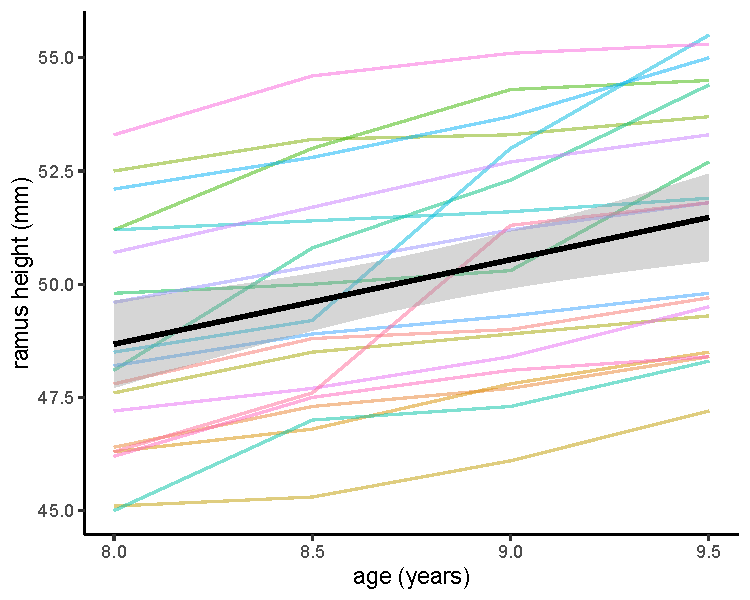
\includegraphics[width=0.6\linewidth]{figs_L2/unnamed-chunk-5-1} \end{center}

\tiny
\end{frame}

\begin{frame}[fragile]{}
\protect\hypertarget{section-3}{}
\tiny

\begin{Shaded}
\begin{Highlighting}[]
\NormalTok{ramus\_s }\OtherTok{\textless{}{-}} \FunctionTok{cbind}\NormalTok{(ramus\_mean, ramus\_sd, }
\NormalTok{                 ramus\_se, }\StringTok{\textasciigrave{}}\AttributeTok{age (years)}\StringTok{\textasciigrave{}}\NormalTok{) }\SpecialCharTok{\%\textgreater{}\%}
  \FunctionTok{as.data.frame}\NormalTok{() }\SpecialCharTok{\%\textgreater{}\%}
  \FunctionTok{mutate\_all}\NormalTok{(as.numeric) }\SpecialCharTok{\%\textgreater{}\%}
  \FunctionTok{round}\NormalTok{(}\DecValTok{4}\NormalTok{) }

\NormalTok{plot1 }\SpecialCharTok{+} \FunctionTok{geom\_line}\NormalTok{(}\AttributeTok{data =}\NormalTok{ ramus\_s, }
                  \FunctionTok{aes}\NormalTok{(}\AttributeTok{x =} \StringTok{\textasciigrave{}}\AttributeTok{age (years)}\StringTok{\textasciigrave{}}\NormalTok{, }
                      \AttributeTok{y =}\NormalTok{ ramus\_mean)) }\SpecialCharTok{+}
  \FunctionTok{geom\_errorbar}\NormalTok{(}\AttributeTok{data =}\NormalTok{ ramus\_s,}
                \FunctionTok{aes}\NormalTok{(}\AttributeTok{x =} \StringTok{\textasciigrave{}}\AttributeTok{age (years)}\StringTok{\textasciigrave{}}\NormalTok{, }\AttributeTok{y =}\NormalTok{ ramus\_mean,}
                    \AttributeTok{ymin =}\NormalTok{ ramus\_mean}\DecValTok{{-}2}\SpecialCharTok{*}\NormalTok{ramus\_se,}
                    \AttributeTok{ymax =}\NormalTok{ ramus\_mean}\SpecialCharTok{+}\DecValTok{2}\SpecialCharTok{*}\NormalTok{ramus\_se),}
                \AttributeTok{width =} \FloatTok{0.05}\NormalTok{,  }\AttributeTok{position =} \FunctionTok{position\_dodge}\NormalTok{(}\FloatTok{0.05}\NormalTok{)) }\SpecialCharTok{+}
  \FunctionTok{theme\_classic}\NormalTok{() }\SpecialCharTok{+}
  \FunctionTok{theme}\NormalTok{(}\AttributeTok{legend.position =} \StringTok{"none"}\NormalTok{) }
\end{Highlighting}
\end{Shaded}

\begin{center}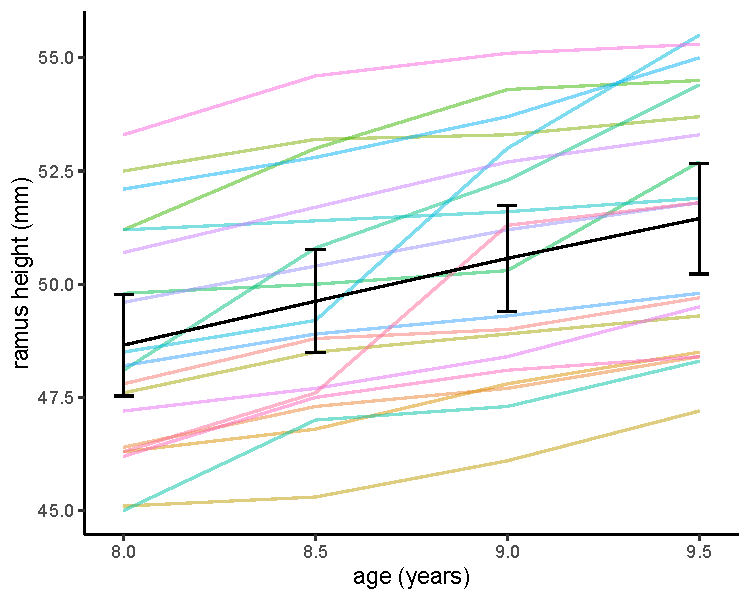
\includegraphics[width=0.6\linewidth]{figs_L2/unnamed-chunk-6-1} \end{center}

\tiny
\end{frame}

\hypertarget{scatterplots}{%
\section{Scatterplots}\label{scatterplots}}

\begin{frame}{Graphs for repeated measures data with multiple samples}
\protect\hypertarget{graphs-for-repeated-measures-data-with-multiple-samples}{}
\begin{itemize}
\tightlist
\item
  Multiple samples present a whole new set of issues when constructing
  graphs.\\
\item
  Consider a simple generic data set with 2 groups (e.g., men, women),
  where individuals are monitored over time.
\item
  The curves are obtained from PROC MIXED, a procedure that we'll learn
  more about later. For now, it is enough to understand that it yields
  predicted values based on the function in the MODEL statement. \tiny
\end{itemize}

\begin{center}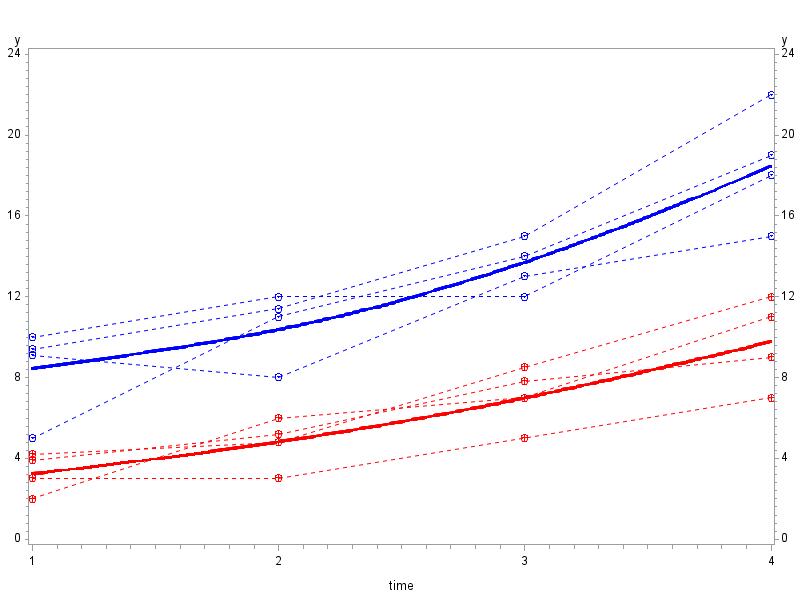
\includegraphics[width=0.6\linewidth]{figs_L2/L2-f1} \end{center}

\tiny
\end{frame}

\begin{frame}{SAS code used to obtain the preceding graph}
\protect\hypertarget{sas-code-used-to-obtain-the-preceding-graph}{}
\tiny

\begin{center}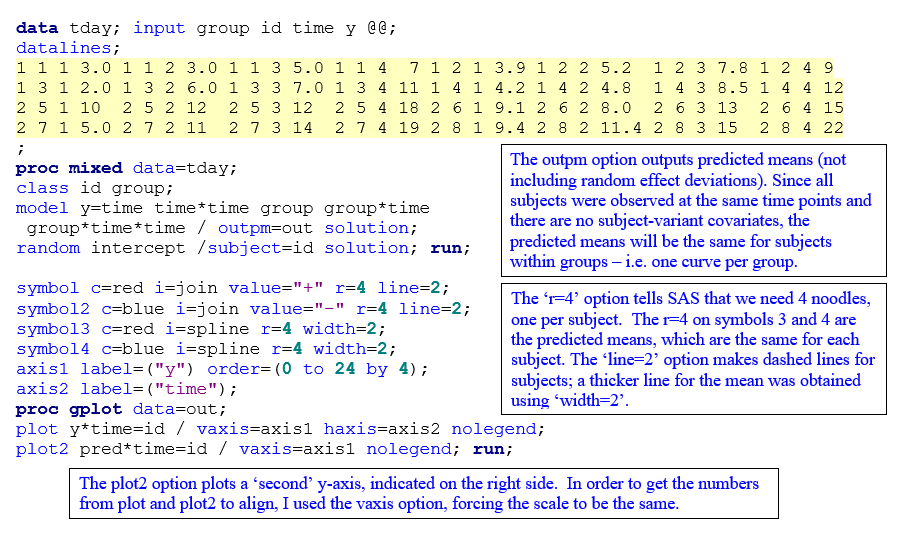
\includegraphics[width=1\linewidth]{figs_L2/L2-f2} \end{center}

\tiny
\end{frame}

\begin{frame}{}
\protect\hypertarget{section-4}{}
\begin{itemize}
\tightlist
\item
  Graphing in SAS has become somewhat easier via the SGPLOT, which
  mimics some of the features that R graphing has.\\
  -Below is a spaghetti plot of the same data. Note the minimal amount
  of coding required to get the plot.\\
\item
  The `reg' statement would allow for plotting of group means, and the
  `degree' option can be added to get polynomial curves.\\
\item
  See the SAS Help Documentation for more detail.
\end{itemize}

\tiny

\begin{center}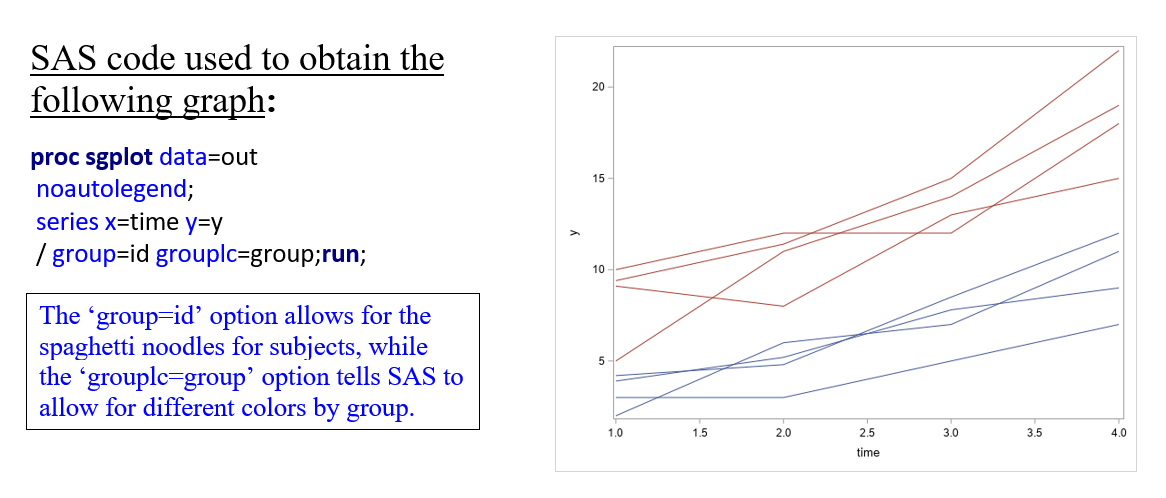
\includegraphics[width=1\linewidth]{figs_L2/L2-f3} \end{center}

\tiny
\end{frame}

\begin{frame}{Graphs for large amounts of data}
\protect\hypertarget{graphs-for-large-amounts-of-data}{}
\begin{itemize}
\item
  With large amounts of longitudinal data, a question arises as to the
  best way to present the data for visual appeal and to best allow for
  interpretations.
\item
  Diggle, et al., (Analysis of Longitudinal Data; 1994, 1996) discuss
  approaches to create graphs for a large data set from the Multicenter
  AIDS Cohort Study (MACS).
\item
  Some of Diggle et al.'s graphing concepts are used here, for data
  involving subjects with idiopathic pulmonary fibrosis (IPF) analyzed
  at NJH.
\item
  The outcome `\% predicted diffusing capacity of the lung' was measured
  on 321 IPF subjects, both before and after diagnosis. This measure
  tends to decrease as subjects progress in their illness (see Strand et
  al., 2014).
\end{itemize}
\end{frame}

\hypertarget{typical-spaghetti-plot-for-the-data.}{%
\section{Typical spaghetti plot for the
data.}\label{typical-spaghetti-plot-for-the-data.}}

\begin{frame}{Typical spaghetti plot for the data.}
\tiny

\begin{center}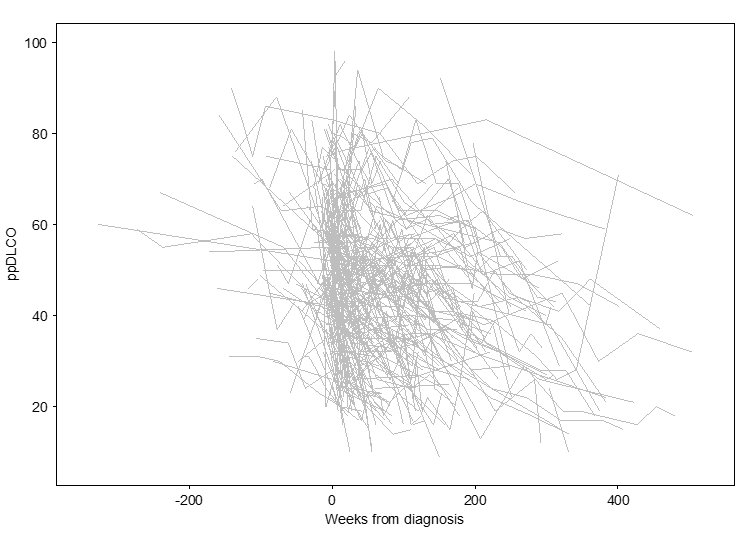
\includegraphics[width=0.6\linewidth]{figs_L2/L2-f4} \end{center}

\tiny
\end{frame}

\begin{frame}{Alternative local polynomial regression}
\protect\hypertarget{alternative-local-polynomial-regression}{}
An alternative to the spaghetti plot is to use symbols for subject-day
values rather than connecting them, and then overlaying the mean
function. Here, local polynomial regression was used to get the fitted
function, using order 1 and a span parameter value of 0.5.

\tiny

\begin{center}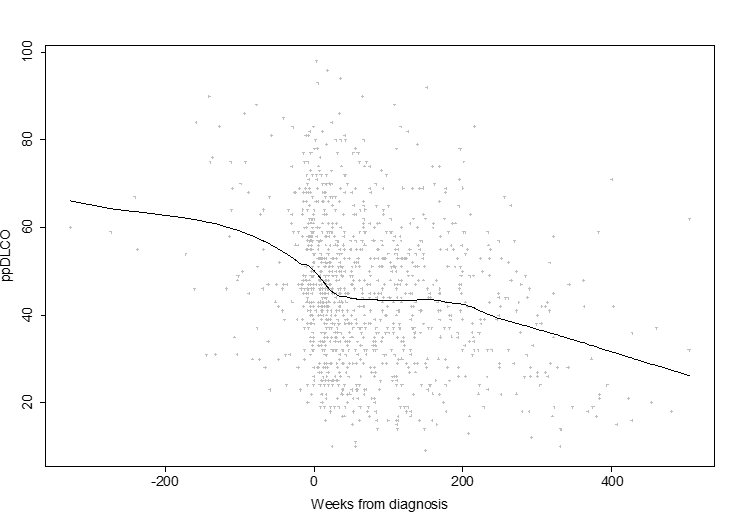
\includegraphics[width=0.6\linewidth]{figs_L2/L2-f5} \end{center}

\tiny
\end{frame}

\begin{frame}{Scatterplot with selective subject trajectory}
\protect\hypertarget{scatterplot-with-selective-subject-trajectory}{}
Scatterplot of IPF data with line graph of 9 randomly selected subjects.

\tiny

\begin{center}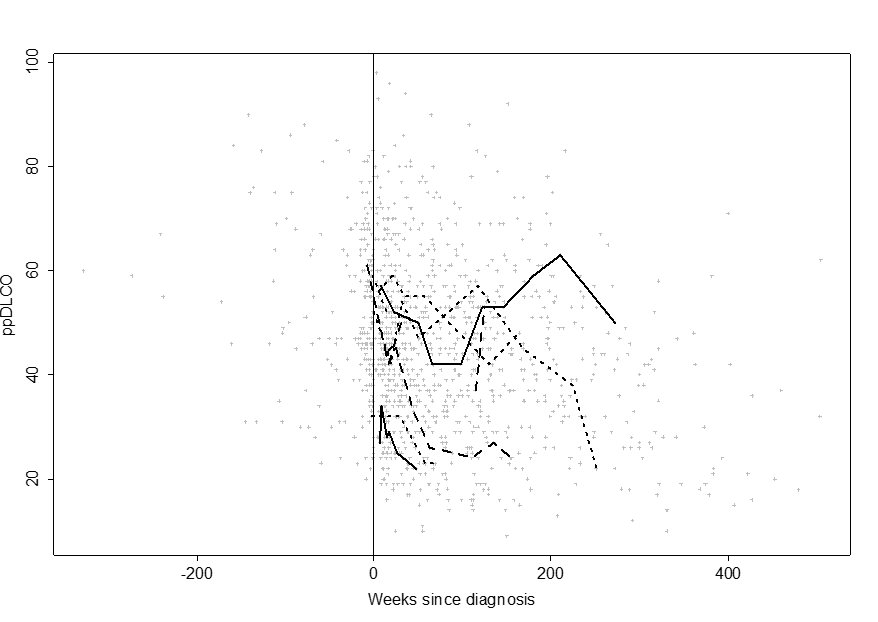
\includegraphics[width=0.75\linewidth]{figs_L2/L2-f6} \end{center}

\tiny
\end{frame}

\begin{frame}{Systematically selected subjects}
\protect\hypertarget{systematically-selected-subjects}{}
Scatterplot of IPF data with line graph of systematically selected
subjects.

The selection of subjects for Figure 2 was as follows:

(i). residuals were calculated for each data point based on
nonparametric regression fit in Figure 1;

(ii). for each subject, the mean residual was determined;

(iii). line segments were included for subjects with certain percentiles
for the mean residual variable. \tiny

\begin{center}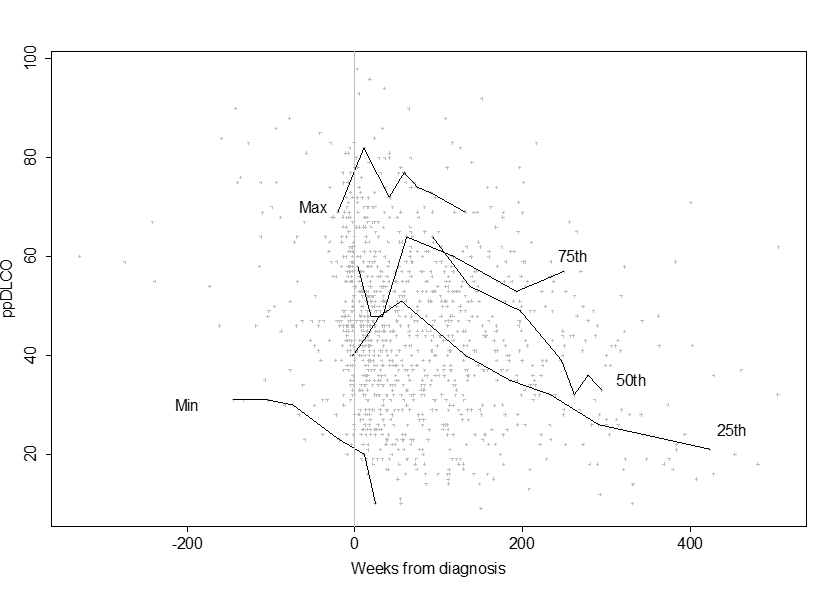
\includegraphics[width=0.65\linewidth]{figs_L2/L2-f7} \end{center}

\tiny
\end{frame}

\hypertarget{graphs-that-display-between--or-within-subject-variability}{%
\section{Graphs that display between- or within-subject
variability}\label{graphs-that-display-between--or-within-subject-variability}}

\begin{frame}{Graphs that display between- or within-subject
variability}
\begin{itemize}
\tightlist
\item
  Mean estimates at individual time points are often graphed including
  `error bars.'
\item
  Consider the data from clinical trial reported in Katial et
  al.~(2010).\\
\item
  Subjects allergic to aspirin were given an aspirin desensitization
  test over 1 day period.\\
\item
  Several measures were taken immediately before (BL) and after
  (post-BL) the desensitization, one being exhaled nitric oxide (eNO).
  Some subjects also had measures at 6 months.
\item
  The following graph displays estimates at individual time points, with
  confidence intervals (CI), based on a linear mixed model (LMM) fit.\\
\item
  \textbf{Are the means at BL and Post-BL time points significantly
  different?} Tests for differences give a \(p=0.025\) for the
  difference b/w the BL and post-BL, and \(p=0.40\) b/w the Bl and 6
  months.\\
  \tiny
\end{itemize}

\begin{center}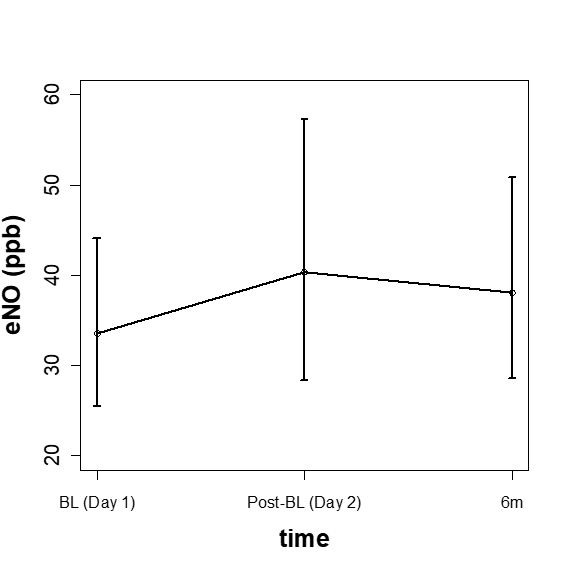
\includegraphics[width=0.32\linewidth]{figs_L2/L2-f8} \end{center}

\tiny
\end{frame}

\begin{frame}{}
\protect\hypertarget{section-5}{}
\begin{itemize}
\item
  The previous graph does not demonstrate variability of within-subject
  changes over time that may be quite different than the SDs of the
  individual time points.
\item
  This graph shows the variability of the difference estimates. Graphed
  are relative change estimates, which result since analysis of eNO was
  on the natural log scale; also plotted in the graph are 95\% CI's for
  these relative estimates.\\
  \tiny
\end{itemize}

\begin{center}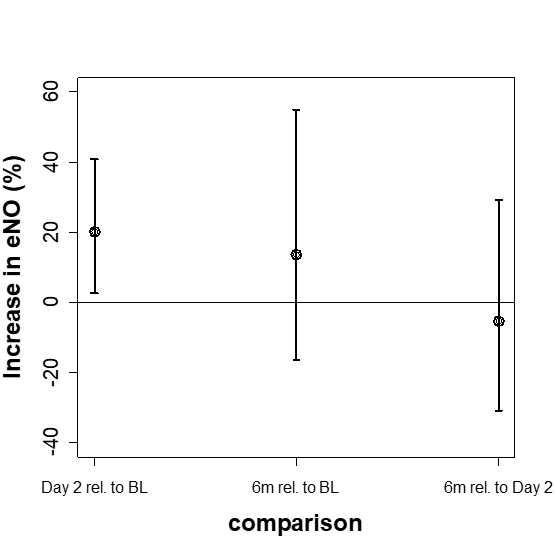
\includegraphics[width=0.4\linewidth]{figs_L2/L2-f9} \end{center}

\tiny

\tiny

Note in the first position of the graph we have the Day 2 estimate
relative to BL, and the CI does not contain 0, which is consistent with
\(p=0.025\) (since we constructed a 95\% CI).

(In this graph the difference estimates are not joined with a line since
the x-axis is not time, but rather it is the comparison of pairs of time
points (one relative to another). (A reference line at \(y=0\) is
included.)
\end{frame}

\hypertarget{lasagna-plots}{%
\section{Lasagna plots}\label{lasagna-plots}}

\begin{frame}{Lasagna plots}
While we're on the topic of Italian food, a `lasagna plot' is an
alternative to the spaghetti plot (See Lasagna plots: a saucy
alternative to spaghetti plots, Bruce Swihart et al., 2010, Epidemiology
21: 621-625.) \tiny

\begin{center}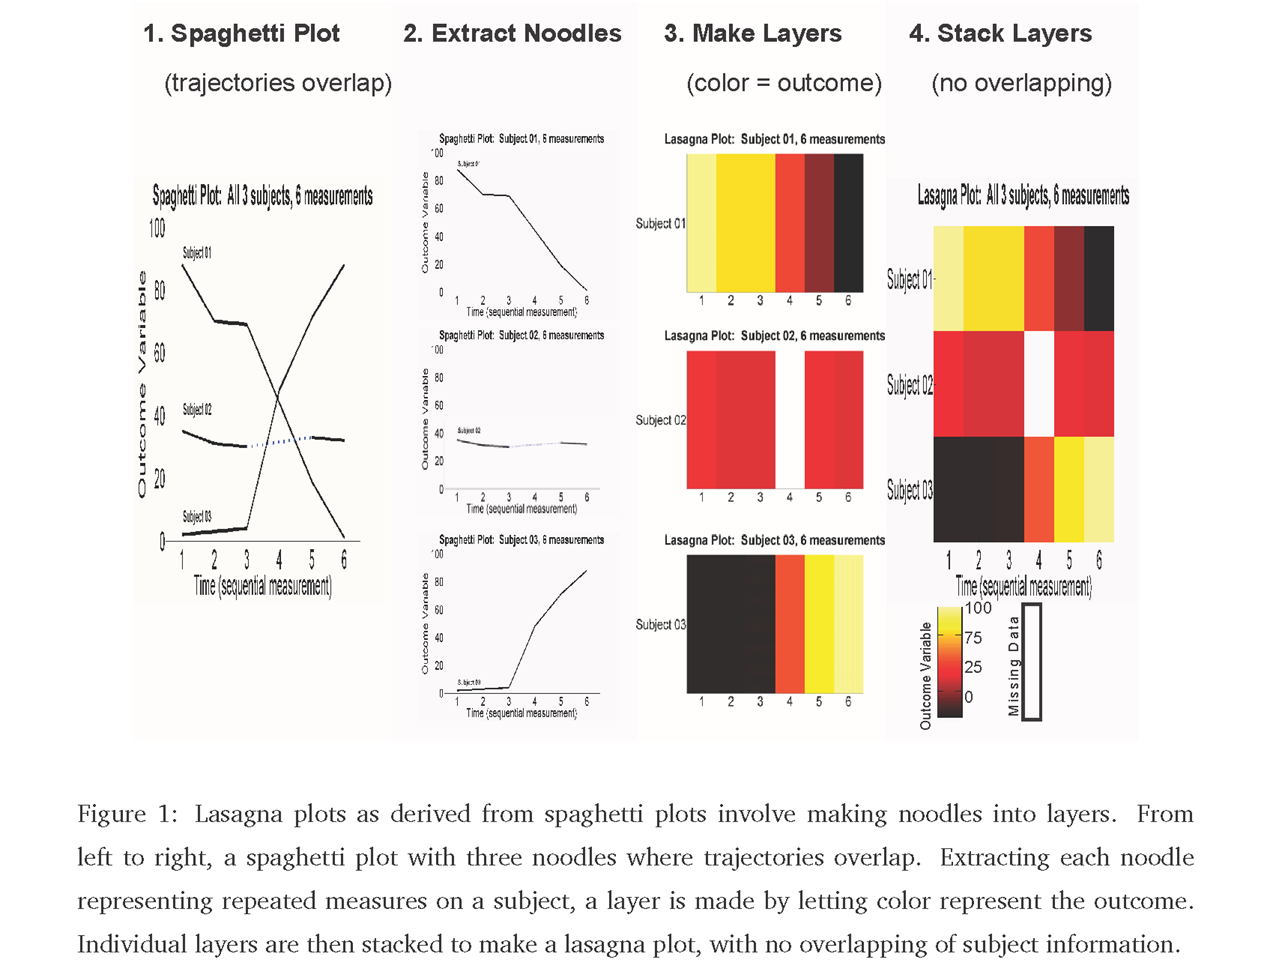
\includegraphics[width=0.85\linewidth]{figs_L2/L2-f10} \end{center}

\tiny
\end{frame}

\hypertarget{pace-charts}{%
\section{Pace charts}\label{pace-charts}}

\begin{frame}{Pace charts}
The last ``0.2'' miles of the 26.2 mile race was adjusted per mile
distance, and shows that although the runner `hit the wall' in the last
3 to 5 miles, he was able to finish strong. The finish time was 3 hours
and 6 minutes.

\tiny

\begin{center}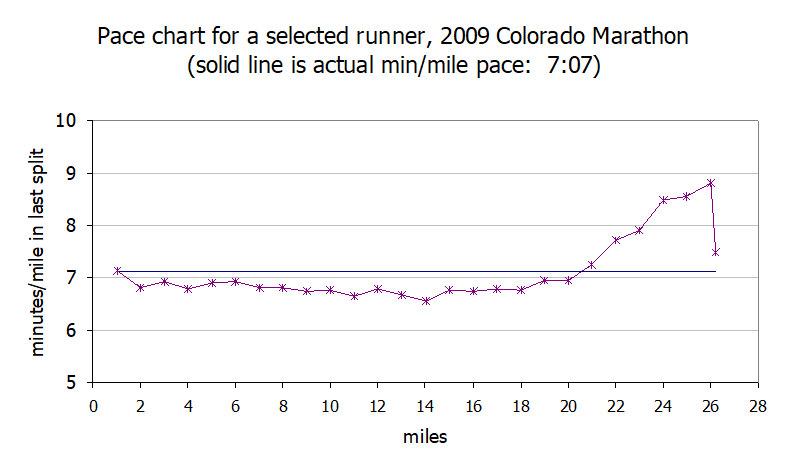
\includegraphics[width=0.6\linewidth]{figs_L2/L2-f11} \end{center}

\tiny
\end{frame}

\begin{frame}{}
\protect\hypertarget{section-6}{}
\tiny

\begin{center}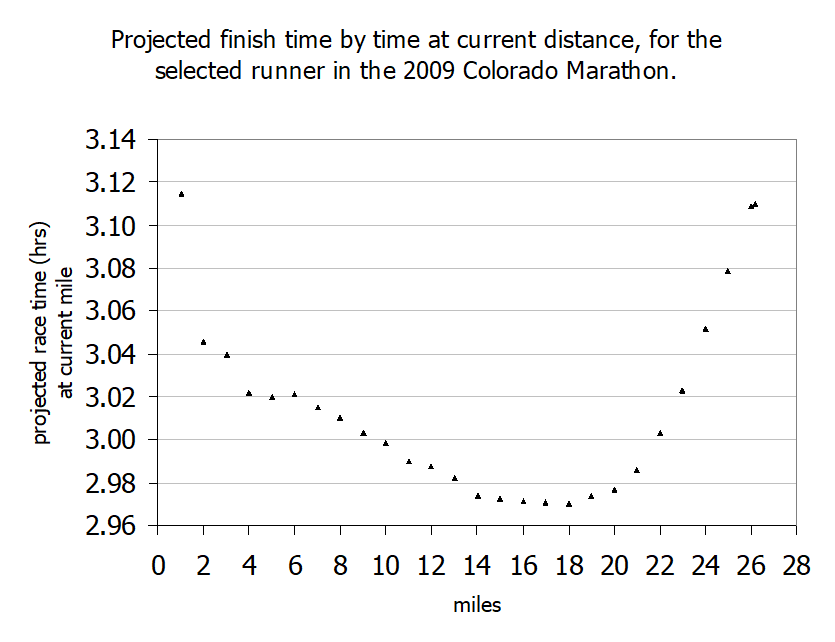
\includegraphics[width=0.6\linewidth]{figs_L2/L2-f12} \end{center}

\tiny
\end{frame}

\hypertarget{graphs-for-unequally-spaced-data-with-common-time-points}{%
\section{Graphs for unequally spaced data with common time
points}\label{graphs-for-unequally-spaced-data-with-common-time-points}}

\begin{frame}{Graphs for unequally spaced data with common time points}
\begin{itemize}
\tightlist
\item
  A longitudinal experiment was conducted by Sorensen et al.~(2003,
  JACI) where measurements were taken at unequally spaced times.
\item
  This experiment involved complement split products, which are
  biological markers measured in the body that may be related to
  symptoms of chronic fatigue syndrome.
\item
  This research aimed at determining which complements correlated with
  symptoms induced with exercise and allergen challenges. One such
  complement was ``C4a''.
\item
  Estimates of geometric mean C4a levels before and after exercise
  challenge for chronic fatigue syndrome (CFS) and Control populations,
  are presented in the following graphs, with 95\% confidence intervals.
  Data were analyzed on the log scale and then inverted back for
  presentation, resulting in a longer upper bars than lower.
\end{itemize}
\end{frame}

\begin{frame}{CFS data, time points presented as equally-spaced
categories}
\protect\hypertarget{cfs-data-time-points-presented-as-equally-spaced-categories}{}
\tiny

\begin{center}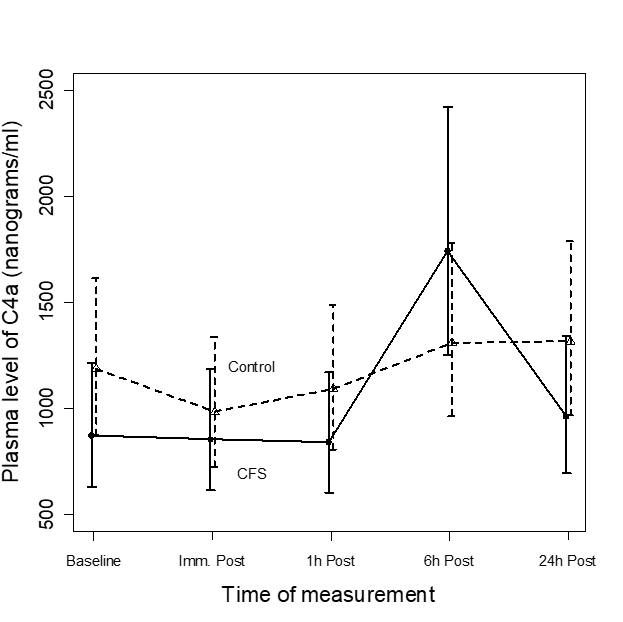
\includegraphics[width=0.6\linewidth]{figs_L2/L2-f13} \end{center}

\tiny
\end{frame}

\begin{frame}{}
\protect\hypertarget{section-7}{}
CFS data, time as metric variable. This is a time-metric sensitive graph
with the same data. Clearly the concentration of data on the left side
makes it difficult to see what is going on.

\tiny

\begin{center}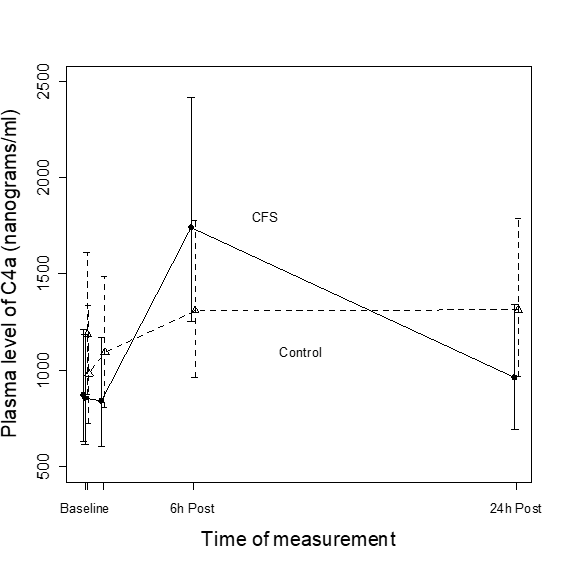
\includegraphics[width=0.6\linewidth]{figs_L2/L2-f14} \end{center}

\tiny
\end{frame}

\begin{frame}{}
\protect\hypertarget{section-8}{}
This is the same basic display, but suppressing CI's for the 2nd and 3rd
time points. Which of the 3 graphs is best?

\tiny

\begin{center}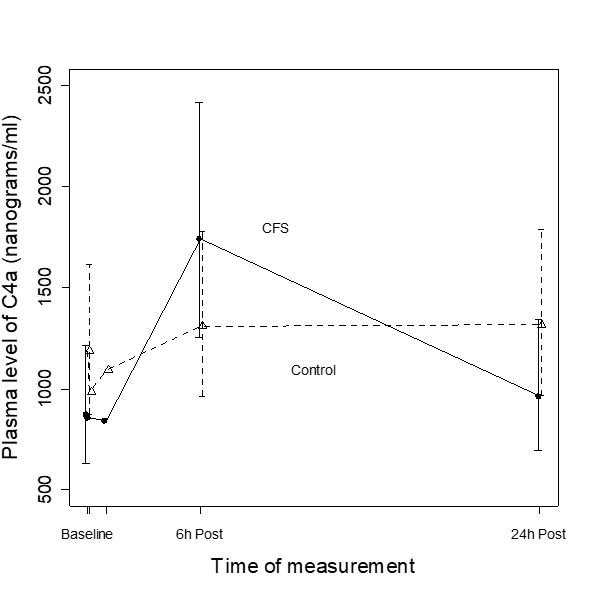
\includegraphics[width=0.6\linewidth]{figs_L2/L2-f15} \end{center}

\tiny

\textbf{See arrow plots in notes}
\end{frame}

\hypertarget{principal-components-analysis-pca}{%
\section{Principal components analysis
(PCA)}\label{principal-components-analysis-pca}}

\begin{frame}{Fundamentals of PCA}
\protect\hypertarget{fundamentals-of-pca}{}
\begin{itemize}
\tightlist
\item
  Principal components analysis is a descriptive tool for longitudinal
  data
\item
  PCA becomes particularly useful for very large data sets with multiple
  variables as a data reduction technique or to find important patterns.
\item
  PCA is used in genetic data analyses, pattern recognition data, growth
  curve analysis, and even with meteorological data to identify
  important climate change patterns.
\item
  PCA is related to factor analysis (FA). In FA, the primary goal is to
  determine latent `factors' in the data. While PCA tends to be more of
  a descriptive technique, FA uses factor rotations of create a reduced
  set of factors that typically have even stronger patterns than
  \(PC\)'s; the remaining unexplained variation is attributed to error.
\end{itemize}
\end{frame}

\begin{frame}{Eigendecomposition}
\protect\hypertarget{eigendecomposition}{}
\begin{itemize}
\tightlist
\item
  Let
  \(\pmb Y = (Y_1,\ Y_2,\ ...,\ Y_r)^{\top} \sim \mathcal {Normal}_r(\pmb \mu, \pmb \Sigma)\)
\end{itemize}

\[
\sum_{i=1}^rVar[Y_i] = trace(\pmb \Sigma)
= trace(\Lambda) = \sum^r_{i=1} Var[PC_i]
\]

\begin{itemize}
\tightlist
\item
  where
  \(\pmb \Sigma_{r \times r} = \pmb {P}_{r \times r} \pmb {\Lambda}_{r \times r} \pmb P^{\top}_{r \times r}\),
  \(\pmb P = (\pmb e_1,\ ...,\ \pmb e_r)\); \(\pmb \Lambda\) is the
  diagonal matrix of eigenvalues, \(\pmb e_i\)s are eigenvectors.
  \textbf{(see the eigen-decomposition section in the Matrix notes)}
\item
  Note the number of eigen vectors (and values) is the same as the
  number of variables (\(r\)).
\item
  The quantity \(\frac {\lambda_i} {\sum \lambda_j}\) indicates the
  proportion of variability in the data accounted for by \(PC_i\).
\item
  In principal components analysis:

  \begin{itemize}
  \tightlist
  \item
    Eigenvalues indicate magnitude of variances of the principle
    components (\(PC\)'s)
  \item
    Eigenvectors indicate direction of the \(PC\)'s.
  \end{itemize}
\end{itemize}
\end{frame}

\begin{frame}{Example: Aspirin/eNO data}
\protect\hypertarget{example-aspirineno-data}{}
\begin{itemize}
\tightlist
\item
  Subjects with aspirin allergies; outcome is eNO pre and post
\item
  Aspirin/eNO data, pre and post-aspirin challenge variables

  \begin{itemize}
  \tightlist
  \item
    Only 2 variables, hence only 2 principle components
  \item
    Somewhat unusual to perform a PCA on only 2 variables
  \item
    Done here primarily for pedagogical purposes, although even a PCA
    for descriptive analysis purposes that uses only 2 variables can be
    helpful!
  \end{itemize}
\item
  \(PC_1 = \pmb e_1^{\top} \begin{pmatrix} Y_1\\ Y_2 \end{pmatrix}\),
  \(PC_2 = \pmb e_2^{\top} \begin{pmatrix} Y_1\\ Y_2 \end{pmatrix}\),
  where \(\pmb e_1\) and \(\pmb e_2\) are the eigenvectors associated
  with \(\lambda_1\) and \(\lambda_2\), respectively, where
  \textcolor{magenta}{$\lambda_1 \leq \lambda_2$}, and \(Y_1\) and
  \(Y_2\) are the original variables.
\end{itemize}

\[
\begin{cases}
PC_1 = 0.51 Y_1 + 0.86 Y_2 \\
PC_2 = -0.86 Y_1 + 0.51 Y_2
\end{cases}
\]
\end{frame}

\begin{frame}{}
\protect\hypertarget{section-9}{}
\begin{itemize}
\tightlist
\item
  Scatterplot of pre and post challenge eNO values.
\item
  A confidence ellipse has been superimposed. Note that the long side of
  the ellipse extends in the direction of \(PC1\), while 90 degrees to
  that is \(PC2\).
\item
  \(PC1\) is a weighted average eNO value (with a higher weight given to
  the post measurement, since it contained more variability); well call
  \(PC1\) the `average' component.
\item
  \(PC2\) differentiates pre \((Y1)\) and post \((Y2)\) eNO values;
  subjects with relatively low values did not react as strongly to the
  aspirin challenge, while subjects with higher values had post \((Y2)\)
  measurements that were much higher than pre measurements. For this
  reason, we can call \(PC2\) the `reactivity' component. \tiny
\end{itemize}

\begin{center}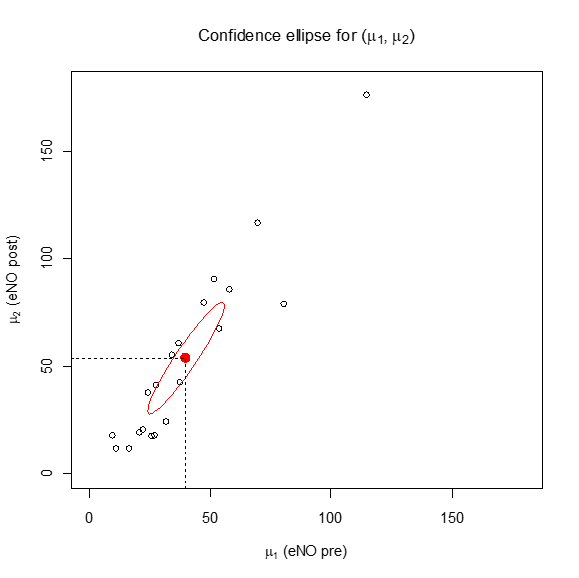
\includegraphics[width=0.4\linewidth]{figs_L2/L2-f19} \end{center}

\tiny
\end{frame}

\begin{frame}{}
\protect\hypertarget{section-10}{}
This scatterplot is really the same as the previous one (with the
confidence ellipse); it is just tilted and stretched.

\begin{itemize}
\tightlist
\item
  It allows us to see some patterns that we wouldn't otherwise see so
  easily. In particular, the subject to the far left could be considered
  an outlier on the reactivity component (\(PC2\)).
\item
  If we go back to the original values, we see that their pre eNO value
  was 80.5, and post value was 79.1, which is unusual because after the
  aspirin challenge, we would expect most subjects to increase in eNO,
  particularly those with higher starting values.
\end{itemize}

\tiny

(Some other subjects also had drops in eNO, but they were ones that had
smaller pre eNO values -- the lower middle scores on the plot.

\tiny

\begin{center}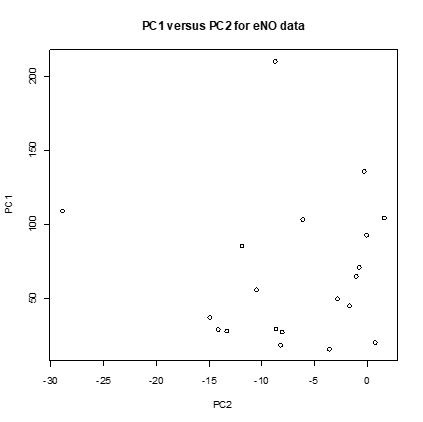
\includegraphics[width=0.5\linewidth]{figs_L2/L2-f20} \end{center}

\tiny
\end{frame}

\begin{frame}{}
\protect\hypertarget{section-11}{}
\begin{itemize}
\tightlist
\item
  The data shows that in fact it was unusual. Those on the far right
  were more common. Another point that stands out is the high point on
  \(PC1\) -- the subject had a very `average' eNO value and did in fact
  increase from pre to post.\\
\item
  Note that there are several different ways that \(PC\)'s can be
  standardized. For example, in SAS, \(PC\)'s are mean corrected. In the
  previous plot, no standardization was done.
\end{itemize}
\end{frame}

\begin{frame}{The Ramus data}
\protect\hypertarget{the-ramus-data}{}
The Ramus data - Ramus bone in the jaw for boys. Each boy was measured
at 8, 8.5, 9, and 9.5 years. The following SAS code can be used to carry
out a standard PCA. \tiny

\begin{center}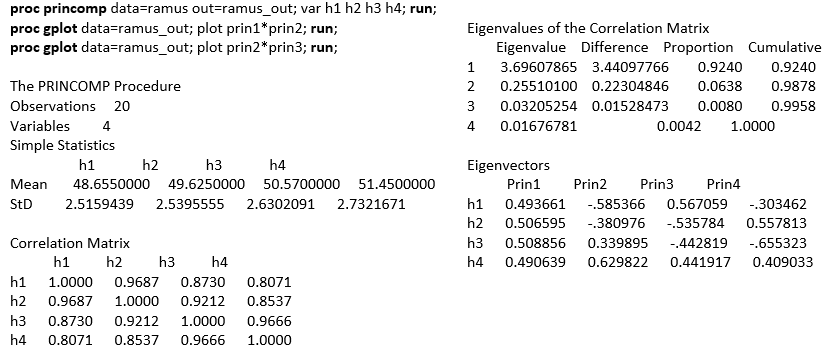
\includegraphics[width=0.86\linewidth]{figs_L2/f22} \end{center}

\tiny
\tiny

\begin{center}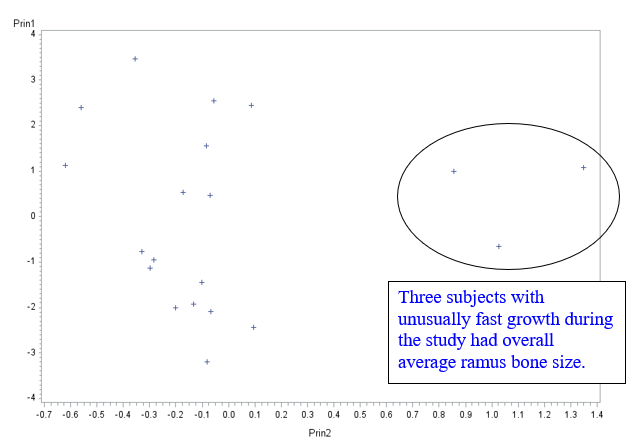
\includegraphics[width=0.5\linewidth]{figs_L2/f21} \end{center}

\tiny
\end{frame}

\begin{frame}{}
\protect\hypertarget{section-12}{}
Original line graph of data, with markers to 3 subjects with unusually
large growth. These subjects are the same as those 3 on the right side
of the previous graph.

\tiny

\begin{center}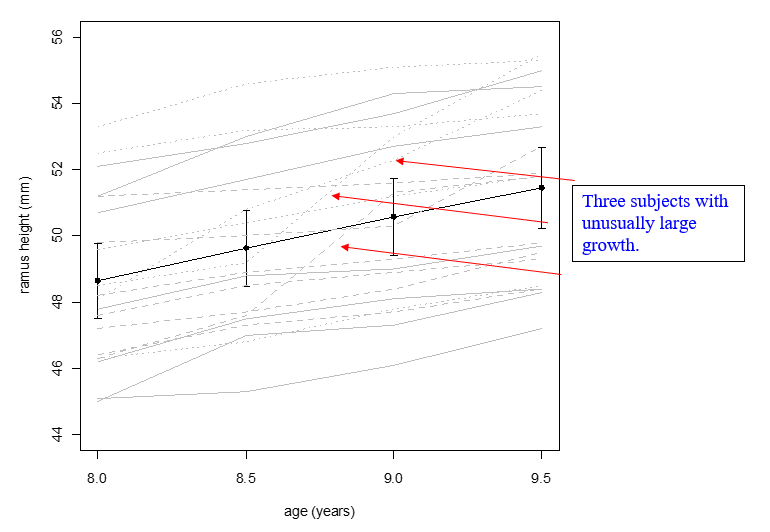
\includegraphics[width=0.95\linewidth]{figs_L2/f23} \end{center}

\tiny
\end{frame}

\begin{frame}{}
\protect\hypertarget{section-13}{}
Plot of \(PC2\) versus \(PC3\). This graph further breaks down the kids
with unusual large growth into those with a quadratic trend (1 subject)
and those without stronger quadratic trend (2 on the left). Also see the
previous graph.

\tiny

\begin{center}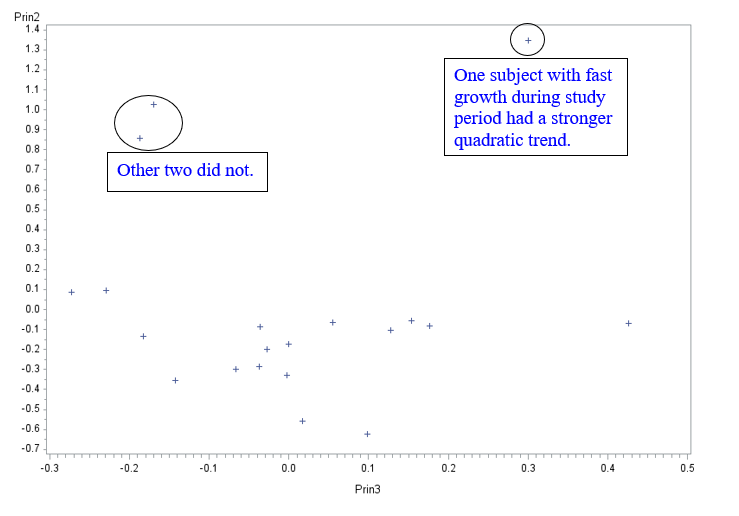
\includegraphics[width=0.8\linewidth]{figs_L2/f24} \end{center}

\tiny
\end{frame}

\begin{frame}{}
\protect\hypertarget{section-14}{}
We can also identify subjects with stronger values of \(PC3\) and
\(PC4\) on the original line graph. (Other subjects are removed in order
to see patterns more clearly.

This PCA allowed us to see quickly subjects with more unusual trends. It
also showed us that the variability in the data is captured through
orthogonal polynomial trends, with decreasing variability as the order
increases (from `intercept' to cubic); nearly 99\% of the
between-subject variability could be captured by the `intercept' and
`linear' components.

\tiny

\begin{center}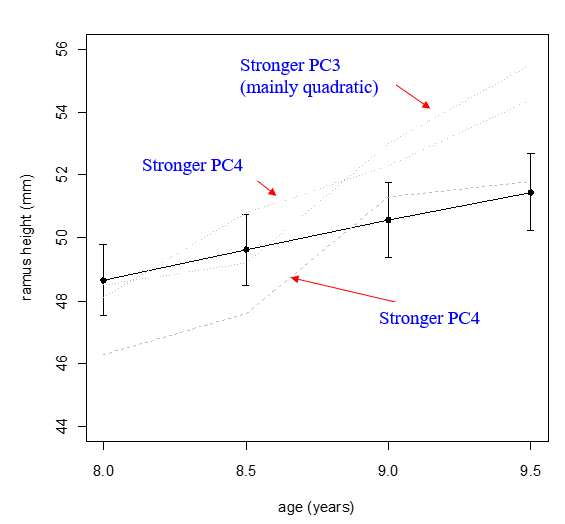
\includegraphics[width=0.6\linewidth]{figs_L2/f25} \end{center}

\tiny
\end{frame}

\hypertarget{summary}{%
\section{Summary}\label{summary}}

\begin{frame}{Summary}
\protect\hypertarget{summary-1}{}
\begin{itemize}
\tightlist
\item
  Line graphs/ spaghetti plots
\item
  Scatterplots
\item
  Graphs that show between and within-subject variability
\item
  Lasagna plot, pace chart, graphs for unequally spaced data
\item
  PCA
\end{itemize}
\end{frame}

\end{document}